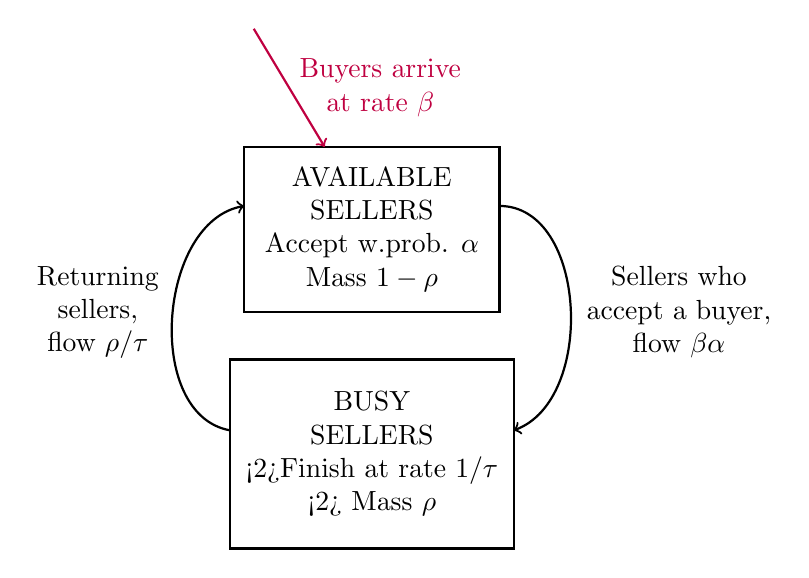
\begin{tikzpicture}[xscale=.6,yscale=.6,xshift=1,yshift=1] 


%	\draw[step=1cm,gray,very thin] (0,0) grid (10,8);




	\draw[thick] (-.2,4) rectangle (5.2,7.5);
	\node at (2.5,5.75) [align=center]  {AVAILABLE\\SELLERS\\Accept w.prob. $\alpha$\\Mass $1-\rho$};

	\draw[thick] (-.5,-1) rectangle (5.5,3);
	\node at (2.5,1) [align=center] {BUSY\\SELLERS\\ {\uncover<2>{Finish at rate $1/\tau$}}\\ {\uncover<2> {Mass $\rho$}}};
	
	


	\draw[thick,->,purple] (0,10) --node[align=center,right] {Buyers arrive\\at rate $\beta$} (1.5,7.5);


	\node at (9,4) [align=center] {Sellers who\\accept a buyer,\\flow  $\beta\alpha$};

	\draw[thick,->] (5.2,6.25) to [out=0,in=20] (5.5,1.5);

\pause


	\node at (-3.3,4) [align=center] {Returning\\sellers,\\flow $\rho/\tau$};

	\draw[thick,->] (-.5,1.5) to [out=170,in=-170] (-.2,6.25);


%		\node at (2.5,1) [align=center] { Y \\Y \\ Finish at rate $1/\tau$\\Mass $1-\rho$};



        
\end{tikzpicture}